\documentclass[a4paper, 10pt]{IEEEtran}

\usepackage{graphicx} 
\usepackage{tabularx}
\usepackage{tabulary}
\usepackage{url}       
\usepackage{amsmath} 
\usepackage{amsfonts}
\usepackage{amssymb}
\usepackage{textcomp,gensymb}
\usepackage{gensymb}
\usepackage{float}
\usepackage[hidelinks]{hyperref}
\usepackage[spanish]{cleveref}
\renewcommand{\tablename}{Tabla}
\renewcommand{\figurename}{Figura}
\renewcommand{\refname}{Referencias}

\begin{document}

\title{Aproximación de PI Utilizando el Método Monte Carlo}
\author{José Benavente
\thanks{}}
\markboth{Computación Paralela - Facultad de Ciencias Empresariales - Universidad del Bío-Bío}{}
\maketitle

\maketitle

\begin{abstract}
Este informe describe un algoritmo basado en el método de Monte Carlo para la aproximación del valor de $\pi$. El método utiliza muestras aleatorias dentro de un cuadrado para así poder aproximar la proporción de puntos que caen dentro de las cuatro esquinas que se generan al colocar un circulo dentro dicho cuadrado. El algoritmo se implementa en C++ y hace uso de la librería estándar para la generación de números aleatorios.
\end{abstract}

\section{Introducción}
El número $\pi$ es una de las constantes matemáticas más importantes y aparece en numerosas áreas de las matemáticas, la física y la ingeniería. Sin embargo, calcular $\pi$ con precisión puede ser computacionalmente costoso. El método de Monte Carlo es un enfoque probabilístico que permite obtener una aproximación de $\pi$ usando técnicas de simulación basadas en números aleatorios. En este informe, se presenta un algoritmo que utiliza este método para estimar el valor de $\pi$.

\section{Método de Monte Carlo}
El método de Monte Carlo se basa en generar un conjunto de puntos aleatorios dentro de un espacio conocido (en este caso, un cuadrado de lado 1) y determinar cuántos de esos puntos caen dentro de una región de interés (un cuarto de círculo inscrito en dicho cuadrado). La proporción de puntos que caen dentro del círculo en comparación con el número total de puntos generados nos permite aproximar el valor de $\pi$.

\subsection{Descripción del Algoritmo}
El algoritmo se implementa en C++ y realiza los siguientes pasos:

\begin{itemize}
    \item Se generan dos números aleatorios $x$ e $y$ entre 0 y 1, los cuales representan las coordenadas de un punto en el plano.
    \item Se verifica si el punto $(x, y)$ cae dentro del cuarto de círculo unitario usando la ecuación $x^2 + y^2 \leq 1$.
    \item Se repite este proceso para un número grande de muestras.
    \item La proporción de puntos que caen dentro del círculo se multiplica por 4 para obtener una aproximación de $\pi$, ya que el área del cuadrado es 1 y el área de un cuarto del círculo es $\pi/4$.
\end{itemize}

\pagebreak

A continuación, se muestra un extracto del código de la implementación secuencial del algoritmo.

\begin{verbatim}
double sequential(int n) {
  int count = 0;

  std::default_random_engine generator;
  std::uniform_real_distribution<double> 
    distribution(0.0, 1.0);
  
  for (int i = 0; i < n; ++i) {
    double x = distribution(generator);
    double y = distribution(generator);
    
    if (x * x + y * y <= 1.0) {
      count++;
    }
  }
  
  return 4.0 * count / n;
}
\end{verbatim}

\section{Resultados}
Al ejecutar este algoritmo con un número suficientemente grande de muestras, es posible obtener una aproximación precisa del valor de $\pi$. La precisión mejora a medida que se aumenta el número de muestras. A continuación, se muestran algunos resultados obtenidos al ejecutar el algoritmo:

\begin{table}[H]
    \centering
    \begin{tabular}{|c|c|}
    \hline
    \textbf{Número de muestras} & \textbf{Aproximación de $\pi$} \\
    \hline
    1000 & 3.140 \\
    10,000 & 3.1412 \\
    100,000 & 3.14159 \\
    1,000,000 & 3.141592 \\
    \hline
    \end{tabular}
    \caption{Aproximación de $\pi$ con diferentes números de muestras.}
    \label{tab:results}
\end{table}

\section{Paralelización del Algoritmo}
La implementación secuencial del algoritmo Monte Carlo para la aproximación de $\pi$ se puede optimizar aprovechando la capacidad de procesamiento paralelo. En esta sección, se abordan los puntos clave de la paralelización del algoritmo y se propone una implementación paralela.

\subsection{Identificación de Cuellos de Botella}
El principal cuello de botella en la versión secuencial del algoritmo es la generación y evaluación de puntos aleatorios en el plano. Esta tarea implica una gran cantidad de cálculos repetitivos y es intensiva en cómputo, especialmente a medida que aumenta el número de muestras. Cada punto se genera y evalúa de forma independiente, lo cual representa una oportunidad perfecta para mejorar el rendimiento mediante paralelización.

\subsection{Partes Potencialmente Paralelizables}
La generación de puntos y su verificación para determinar si caen dentro del círculo son tareas independientes entre sí. Esto significa que el cálculo se puede dividir entre múltiples hilos o procesos, sin que el resultado de una iteración afecte a las demás. Por tanto, el bucle principal del algoritmo es altamente paralelizable.

\subsection{Propuesta de Paralelización}
Para la implementación paralela del algoritmo Monte Carlo se utilizará la biblioteca OpenMP, que permite distribuir el bucle principal entre múltiples hilos. Cada hilo generará sus propios puntos aleatorios y contará cuántos de ellos caen dentro del círculo. Al final del cálculo, los resultados parciales de cada hilo se combinarán para obtener la cuenta total de puntos dentro del círculo y calcular el valor de $\pi$. Este enfoque garantiza una distribución de la carga de trabajo y minimiza la contención de recursos.

\subsection{Entorno de Experimentación}
Los experimentos se realizaron en un entorno de hardware y software específico para evaluar el rendimiento de las versiones secuencial y paralelizada del algoritmo. A continuación, se detallan las características de este entorno:

\begin{itemize}
  \item \textbf{Hardware:} Procesador AMD Ryzen 7 3700X de 8 núcleos a 3.6 GHz (modo nominal), con 32 MB de caché L3, 4 MB de caché L2 y 256 KB de caché L1d y L1i. La máquina es virtualizada, utilizando KVM como hipervisor, y cuenta con 8 GB de RAM asignada en un entorno de 64 bits.

  \item \textbf{Sistema operativo:} Debian GNU/Linux 11 (Bullseye).
  
  \item \textbf{Compilador:} GCC versión 9.3.0, con soporte para OpenMP.
  
  \item \textbf{Librerías:} Se utiliza la biblioteca estándar de C++ para la generación de números aleatorios y la biblioteca OpenMP para implementar la paralelización.
  
  \item \textbf{Entorno de desarrollo:} Code::Blocks configurado con targets de perfilado para las versiones secuencial y paralelizada del algoritmo. Las opciones de compilación incluyen `-g` para depuración, `-pg` para generación de perfiles y `-fopenmp` para habilitar la paralelización.
\end{itemize}

Este entorno permite analizar el rendimiento y la escalabilidad de la implementación paralela en comparación con la versión secuencial, evaluando tanto el tiempo de ejecución como la precisión de ambas versiones del algoritmo.

\subsection{Datos de Prueba}
Para analizar el comportamiento de la versión secuencial del algoritmo Monte Carlo, se realizaron pruebas con diferentes cantidades de muestras, variando entre $10$ y $10,000,000$. Estos datos de prueba permiten observar cómo el tiempo de ejecución crece con el número de muestras, proporcionando información relevante sobre la eficiencia del algoritmo. A continuación, se muestran algunos valores utilizados en las pruebas:

\begin{itemize}
  \item $n = 10$
  \item $n = 1000$
  \item $n = 100,000$
  \item $n = 1,000,000$
  \item $n = 10,000,000$
\end{itemize}

Estos valores de $n$ han sido seleccionados para comprender el comportamiento del tiempo de ejecución y la precisión en distintos escenarios.

\subsection{Perfil de los Algoritmos}
Para el análisis de perfil de la versión secuencial, se utilizó la herramienta \texttt{gprof} y se generó un gráfico de distribución de tiempos de ejecución de las funciones. En la \cref{fig:sec_profile} se muestra la imagen obtenida del perfil de las funciones principales.

\begin{figure}[H]
  \centering
  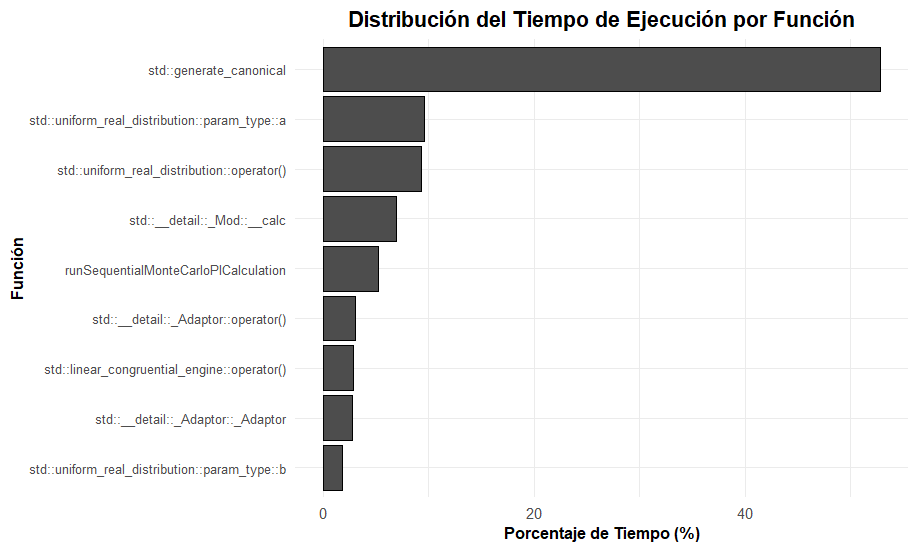
\includegraphics[width=0.5\textwidth]{./img/secuencial.png}
  \caption{Perfil de tiempo de funciones en la versión secuencial.}
  \label{fig:sec_profile}
\end{figure}

Como se observa en la figura, la función que genera números aleatorios, \texttt{std::generate\_canonical}, es la que más tiempo consume, representando aproximadamente el 52.86\% del tiempo total de ejecución. Las funciones asociadas a la distribución aleatoria, como \texttt{std::uniform\_real\_distribution} y \texttt{std::\_\_detail::\_Mod}, también tienen una participación significativa, representando en conjunto alrededor del 30\% del tiempo. La función principal del cálculo secuencial, \texttt{runSequentialMonteCarloPICalculation}, representa cerca del 5.23\% del tiempo de ejecución total.

\subsection{Muestra de Tiempos de Ejecución}
La siguiente tabla presenta los tiempos de ejecución obtenidos en la versión secuencial del algoritmo para diferentes valores de $n$, calculados en un entorno de experimentación específico. Estos valores muestran el crecimiento en el tiempo de ejecución en función del aumento de muestras, lo que se alinea con el comportamiento esperado del método Monte Carlo.

\begin{table}[H]
  \centering
  \begin{tabular}{|c|c|}
    \hline
    \textbf{Número de muestras ($n$)} & \textbf{Tiempo de ejecución (s)} \\
    \hline
    10 & 0.0345 \\
    1,000 & 0.0965 \\
    100,000 & 3.4340 \\
    1,000,000 & 50.3237 \\
    10,000,000 & 8433.2326 \\
    \hline
  \end{tabular}
  \caption{Tiempos de ejecución para diferentes valores de $n$ en la versión secuencial.}
  \label{tab:execution_times}
\end{table}

\subsection{Propuesta de Paralelización e Identificación de Dependencias}
A partir del análisis del perfil, se identifican algunas funciones que serían candidatas ideales para la paralelización. La función \texttt{runSequentialMonteCarloPICalculation}, que realiza la iteración principal, es altamente paralelizable, ya que cada punto generado es independiente de los demás y no afecta el cálculo de otros puntos. Esto permite distribuir las iteraciones entre múltiples hilos sin introducir dependencias entre las operaciones.

En términos de dependencias, la única dependencia importante se encuentra en la acumulación de la cuenta total de puntos dentro del círculo. Para resolver esto, se puede utilizar una reducción en OpenMP, evitando así el uso de operaciones atómicas que puedan introducir contención y reducir el rendimiento. Por lo tanto y para resumir, se propone dividir las iteraciones del cálculo principal y la generación de puntos aleatorios entre hilos, combinando los resultados parciales al final del cálculo.
\end{document}
